\chapter{Analýza a specifikace požadavků}
\label{chap:analyza}

Celý proces analýzy a sběru požadavků probíhal v agilním prostředí. Během vývoje se využívaly iterativní schůzky, pravidelné standupy a dedikované brainstormové sekce. Na těchto setkáních byli přítomni zkušení vývojáři a technický ředitel (CTO), který díky přímému kontaktu se zákazníky detailně znal jejich konkrétní požadavky a tlumočil jejich zpětnou vazbu. Díky tomu bylo možné rychle a efektivně reagovat na potřeby uživatelů a správně specifikovat klíčové vlastnosti aplikace.

\section{Identifikace zúčastněných stran}
Primárními uživateli GoodAccess CLI pro Linux jsou:
\begin{itemize}
    \item \textbf{System Administrators:} Spravují servery a vyžadují stabilní nástroj pro vzdálenou správu přes SSH bez nutnosti grafického rozhraní.
    \item \textbf{DevOps Inženýři:} Potřebují integrovat VPN připojení do automatizovaných skriptů a CI/CD pipelines. Vyžadují predikovatelné chování a strojově čitelný výstup.
    \item \textbf{Běžní zaměstnanci:} Uživatelé, kteří preferují textové uživatelské rozhraní (TUI) před grafickým klientem (GUI) pro každodenní práci.
\end{itemize}

\section{Případy užití}
Hlavní scénáře použití systému z pohledu koncového uživatele (administrátora či běžného zaměstnance) ukazuje následující diagram případů užití (Obrázek \ref{fig:usecase}).

\begin{figure}[H]
    \centering
    \begin{tikzpicture}[scale=1.0, transform shape, font=\sffamily,
        usecase/.style={rectangle, rounded corners=3ex, draw=black, fill=blue!5, text centered, inner sep=2mm, text width=3.5cm, minimum height=1cm},
        actor/.style={draw=none, fill=none, text centered},
        line/.style={-, thick, draw=black!70}]

        % Hranice systému
        \draw[thick, draw=black!50, rounded corners=1ex, fill=gray!5] (-0.5, -4.5) rectangle (4.5, 5.5);
        \node at (2, 5) {\large \textbf{GoodAccess CLI}};

        % Uživatel (stickman)
        \node[actor] (user) at (-3.5, 0.5) {
            \begin{tikzpicture}[scale=0.8]
                \draw[thick] (0,0.5) circle (0.3); % Hlava
                \draw[thick] (0,0.2) -- (0,-0.6); % Tělo
                \draw[thick] (-0.4,-0.1) -- (0.4,-0.1); % Ruce
                \draw[thick] (0,-0.6) -- (-0.4,-1.2); % Levá noha
                \draw[thick] (0,-0.6) -- (0.4,-1.2); % Pravá noha
                \node at (0,-1.6) {\textbf{Uživatel}};
            \end{tikzpicture}
        };

        % Use Cases
        \node[usecase] (setup) at (2, 4) {Prvotní nastavení\\(Setup)};
        \node[usecase] (login) at (2, 2.5) {Přihlášení\\(Login)};
        \node[usecase] (connect) at (2, 1) {Připojení k VPN\\(Connect)};
        \node[usecase] (status) at (2, -0.5) {Zjištění stavu\\(Status)};
        \node[usecase] (disconnect) at (2, -2) {Odpojení VPN\\(Disconnect)};
        \node[usecase] (logout) at (2, -3.5) {Odhlášení\\(Logout)};

        % Vztahy
        \draw[line] (user) -- (setup.west);
        \draw[line] (user) -- (login.west);
        \draw[line] (user) -- (connect.west);
        \draw[line] (user) -- (status.west);
        \draw[line] (user) -- (disconnect.west);
        \draw[line] (user) -- (logout.west);
    \end{tikzpicture}
    \caption{Diagram případů užití GoodAccess CLI}
    \label{fig:usecase}
\end{figure}

\section{Funkční požadavky}
\label{sec:funkcni_pozadavky}
Na základě analýzy potřeb byly stanoveny následující funkční požadavky:

\subsection{Autentizace a správa relace}
Aplikace musí umožnit přihlášení uživatele v prostředí bez webového prohlížeče. Z tohoto důvodu nepodporuje přihlášení pomocí webového SSO (Single Sign-On).
\begin{itemize}
    \item \textbf{F1 -- Login:} Přihlášení probíhá pomocí standardního terminálového vstupu, kam uživatel zadá název týmu, uživatelské jméno a heslo. Zadávání hesla je pro bezpečnost maskováno (zobrazují se pouze znaky \texttt{*}).
    \item \textbf{F2 -- Logout:} Standardní ukončení relace uživatele a bezpečné smazání lokálně uložených tokenů.
    \item \textbf{F3 -- Setup:} Interaktivní průvodce prvotním nastavením (onboarding wizard). Umožňuje uživateli v jednom kroku provést přihlášení, zvolit protokol, vybrat bránu, nastavit perzistentní připojení a rovnou se připojit. Tento proces je striktně interaktivní.
\end{itemize}

\subsection{Správa připojení}
Jádrem aplikace je ovládání VPN tunelu a správa nastavení pro připojení.
\begin{itemize}
    \item \textbf{F4 -- Connect:} Navázání připojení. Standardně se využije preferovaný protokol a brána (gateway) uložená z předchozího nastavení.
    \item \textbf{F5 -- Connect Flags:} Možnost dočasně přepsat preferované nastavení při připojení pomocí přepínačů \texttt{-g} (gateway) a \texttt{-p} (protocol). Přepínač \texttt{--protocol} očekává textový název protokolu, zatímco \texttt{--gateway} vyvolá interaktivní výběr. Tato volba se neuloží jako preferovaná.
    \item \textbf{F6 -- Disconnect:} Korektní ukončení VPN připojení a úklid routovacích pravidel.
    \item \textbf{F7 -- Persistent Connect:} Nastavení připojení na úrovni celého zařízení, které zajistí automatické znovupřipojení i po restartu počítače.
    \item \textbf{F8 -- Gateway Selection:} Možnost uživatele vybrat si konkrétní VPN bránu.
    \item \textbf{F9 -- Protocol Selection:} Možnost uživatele zvolit preferovaný VPN protokol (WireGuard nebo OpenVPN).
\end{itemize}

\subsection{Monitoring a stav}
\begin{itemize}
    \item \textbf{F10 -- Status:} Zobrazení aktuálního stavu připojení (Připojeno/Odpojeno, IP adresa, přenesená data). Výstup lze volitelně formátovat do JSON pro snadné strojové zpracování.
\end{itemize}

\subsection{Obecné příkazy}
\begin{itemize}
    \item \textbf{F11 -- Version:} Zobrazení aktuální verze aplikace.
    \item \textbf{F12 -- Help:} Zobrazení standardní nápovědy k dostupným příkazům a jejich použití.
\end{itemize}

\section{Mimofunkční požadavky}
\label{sec:nefunkcni_pozadavky}
\begin{itemize}
    \item \textbf{M1 -- Výkon a odezva:} Aplikace v prostředí příkazové řádky (CLI) musí reagovat okamžitě. Zásadní je rychlý start aplikace a nízká paměťová náročnost, aby její spuštění uživatele neomezovalo.
    \item \textbf{M2 -- Kompatibilita:} Aplikace musí být funkční na hlavních serverových distribucích Linuxu (Debian/Ubuntu, Fedora/RHEL).
    \item \textbf{M3 -- Bezpečnost:} Citlivá data (přístupové tokeny, privátní klíče) musí být uložena bezpečně a přístupná pouze oprávněné službě.
    \item \textbf{M4 -- Distribuce a nasazení:} Pro usnadnění instalace a správy ze strany systémových administrátorů musí být aplikace zabalitelná do standardních distribučních balíčků. Konkrétně se jedná o formáty \texttt{.deb} (pro rodinu Debian) a \texttt{.rpm} (pro rodinu Red Hat).
\end{itemize}

\section{Analýza architektury}
\label{sec:analyza_architektury}
\subsection{Analýza stávajícího řešení GoodAccess}
Aplikace GoodAccess na operačním systému Linux v současné době funguje jako rozdělený systém složený ze dvou hlavních komponent:

\begin{itemize}
    \item \textbf{GoodAccessService (Daemon):} Tato služba běží na pozadí pod správou systému \texttt{systemd} s právy uživatele \texttt{root}. Její primární odpovědností je správa síťových rozhraní (především tunelů WireGuard), konfigurace systémového směrování (routingu) a bezpečné uchovávání kryptografických klíčů a certifikátů.
    \item \textbf{Grafický klient (Electron/GUI):} Uživatelské rozhraní je postaveno na frameworku Electron. Tato část běží v běžném uživatelském prostoru (bez root oprávnění) a funguje v podstatě jako „hloupý“ prezentační ovladač. Zobrazuje stav a přijímá příkazy od uživatele, které následně předává daemonu ke zpracování. Komunikace mezi těmito dvěma procesy probíhá lokálně, typicky pomocí Unix Domain Sockets (IPC).
\end{itemize}

\subsection{Možné architektonické přístupy}
Při návrhu řešení byly zvažovány dva přístupy k interakci s existující logikou GoodAccess:

\begin{description}
    \item[Návrh A: Tenký klient (Wrapper)] V tomto modelu běží v systému jedna privilegovaná služba (.NET), která drží stav a vykonává operace. CLI aplikace (Go) slouží pouze jako dálkové ovládání, které posílá příkazy službě přes IPC.
    \item[Návrh B: Samostatná logika] CLI aplikace by obsahovala veškerou logiku pro připojení a správu WireGuardu a běžela by přímo pod uživatelem \texttt{root}, nezávisle na existující službě.
\end{description}

\subsection{Zvolené řešení}
Byl zvolen \textbf{Návrh A (Wrapper)} z následujících důvodů:
\begin{enumerate}
    \item \textbf{Single Source of Truth:} Služba drží jednotný stav aplikace. Nedochází k desynchronizaci mezi tím, co si myslí CLI, a tím, co je reálně nastaveno v síti.
    \item \textbf{Bezpečnost:} Uživatel nemusí spouštět CLI pod \texttt{rootem}. Privilegované operace provádí pouze izolovaná služba na pozadí.
    \item \textbf{Znovupoužitelnost:} Využívá se již otestovaná a existující logika v .NET backendu, což je v souladu s hodnotou jednoduchosti (Simplicity) metodiky Extreme Programming (\ref{sec:agile_teorie}).
\end{enumerate}

%\begin{figure}[H]
%    \centering
%    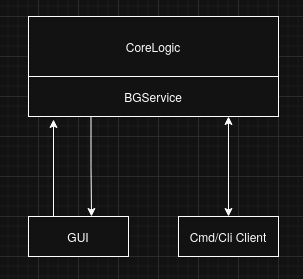
\includegraphics[width=0.8\textwidth]{images/architecture.png}
%    \caption{Zvolená architektura: Tenký klient (Wrapper)}
%    \label{fig:architecture}
%\end{figure}
